\chapter{Оценивание параметров каналов связи с расширенными моделями}\label{ch:ch2}

\section{Оценивание параметров каналов связи в широкополосных системах}\label{ch:ch2/sec1}

% Результаты данного раздела доклада были опубликованы в \cite{Zhang2017, Podkurkov2019}.

Рассмотрим систему с Ортогональным Частотным Разделением Каналов (ОЧРК, англ. OFDM) с одной передающей и массивом приёмных антенн (SIMO).

Использование OFDM модуляции позволяет проектировать инфокоммуникационные системы с двойным назначением - интегрированные системы связи и локации \cite{Sturm09, Sturm10, Sturm11, Braun14}.

В такой системе радиолокационный приёмник находится (приблизительно) в одной точке с передатчиком и интегрирован с ним. Таким образом, при решении задачи локализации отражателей сигналов, локационный приёмник имеет доступ к переданному сигналу $s()$ (уравнение \eqref{eq:ch1:3}).

Учитывая, что количество передающих антенн $\Ntx=1$, уравнения \eqref{eq:ch1:3} и \eqref{eq:ch1:10} в данном случае можно переписать как:

\let\gpai\pai
\let\ggaini\gaini
\let\gdelay\delay
\renewcommand{\pai}{{l}}
\renewcommand{\gaini}{\gain_\pai}
\renewcommand{\delay}{\tau_\pai}
\renewcommand{\vrel}{v_\pai}
\newcommand{\sx}{\Delta_x}
\newcommand{\sy}{\Delta_y}
\newcommand{\rxxi}{\rxi_x}
\newcommand{\rxyi}{\rxi_y}
\newcommand{\dcx}{\nu_\pai^x}
\newcommand{\dcy}{\nu_\pai^y}

\begin{equation}
\label{eq:ch2/sec1:3}
y(\ti,\fri,\rxi) = h(\ti,\fri,\rxi) \cdot s(\ti,\fri) + n(\ti,\fri,\rxi)
\end{equation}
и (учитывая $\gpai=\pai$)
\begin{equation}
\begin{aligned}
\label{eq:ch1/sec1:10}
\hpa(\ti,\fri,\rxi) =&\underbrace{\tgaini \cdot e^{-j2\pi \lfr \delay}}_{\gaini} \cdot 
\underbrace{e^{-j2\pi \scs \fri \delay}}_{b_{\pai,\fri}^f} \cdot
\underbrace{e^{j2\pi \frac{\sfr \ts\ti}{c} \vrel}}_{b_{\pai,\ti,\fri}^t} \cdot
\underbrace{e^{-j2\pi \frac{\sfr}{c} \delrx}}_{b_{\pai,\rxi,\fri}^\te{rx}} \\
=&\gain_{\pai,\txi}^\ti \cdot b_{\pai,\fri}^f \cdot b_{\pai,\ti,\fri}^t  \cdot b_{\pai,\rxi,\fri}^\te{rx}
\end{aligned}
\end{equation}

Примем предположение о работе системы в дальнем поле:
\begin{assumption}
	\label{as:ch2/sec1:1}
	Направление прихода отражённых волн на массив антенн одинаково для каждой приёмной антенны $\rxi$, $\forall$ $0\leq\rxi<\Nrx$.
\end{assumption}

Рассматриваемая система использует \textit{прямоугольный массив антенн с равномерным шагом} (англ. URA - Uniform Rectangular Array), который представляет собой равномерную прямоугольную решётку антенн с одинаковым шагом строк/столбцов этой решётки.

Как видно из уравнений \eqref{eq:ch1:10}, \eqref{eq:ch1:11}, \eqref{eq:ch1/sec1:10}, зависимость коэффициентов $b_{\pai,\ti,\fri}^t$ и $b_{\pai,\rxi,\fri}^\te{rx}$ от частоты (индекс $\fri$) не позволяет прямо применять распространённые алгоритмы оценки параметров канала связи (в том числе направлений прихода сигналов), рассчитанные на узкополосные системы (системы в которых, в виду малой относительной полосы частот $\Bfr$, зависимость от частоты опускается и принимается $\sfr\approx\cfr$ (за исключением коэффициента $b_{\pai,\fri}^f$)) не применимы.

Современные инфокоммуникационные системы стремятся к увеличению пропускной способности за счёт увеличения используемой полосы частот. Поэтому предположение об узкополосности системы тем менее оправдано, чем больше относительная полоса частот системы $\Bfr=\Bw/\cfr$, где $\Bw$ - полоса частот системы. При увеличении $\Bfr$, увеличивается разброс значений $\sfr$, что, в свою очередь, ведёт к увеличению систематической ошибки вносимой предположением $\sfr\approx\cfr$, которая в при больших значениях $\Bfr$ приводит к полной несостоятельности узкополосных алгоритмов.

Для решения этой задачи была предложена методика предварительной обработки получаемых данных, используя которую можно существенно снизить вносимые искажения и, в то же время, сохранить состоятельность узкополосных алгоритмов оценивания при более высоких значениях $\Bfr$. 

Для того, чтобы скомпенсировать зависимость $\sfr$ от частоты, можно обратно-пропорционально изменить интервалы дискретизации в соответствующих измерениях $\ts$ во времени для $b_{\pai,\ti,\fri}^t$ и расстояния между антеннами для $b_{\pai,\rxi,\fri}^\te{rx}$. 

Практически такое изменение означало бы разные аппаратные конфигурации системы для каждой отдельной частоты, однако вместо этого, данные собранные с фиксированными шагами дискретизации во времени и пространстве можно интерполировать для получения данных с необходимыми свойствами.

Интерполирование принятых данных вводит корреляцию между полученными значениями и уменьшает эффективные <<апертуры>> измерений на высоких частотах, поэтому систематическая ошибка не может быть устранена полностью, однако достигается существенное улучшение точности оценивания, особенно при больших значениях $\Bfr$. 

\begin{figure}[ht]
	\centerfloat{
		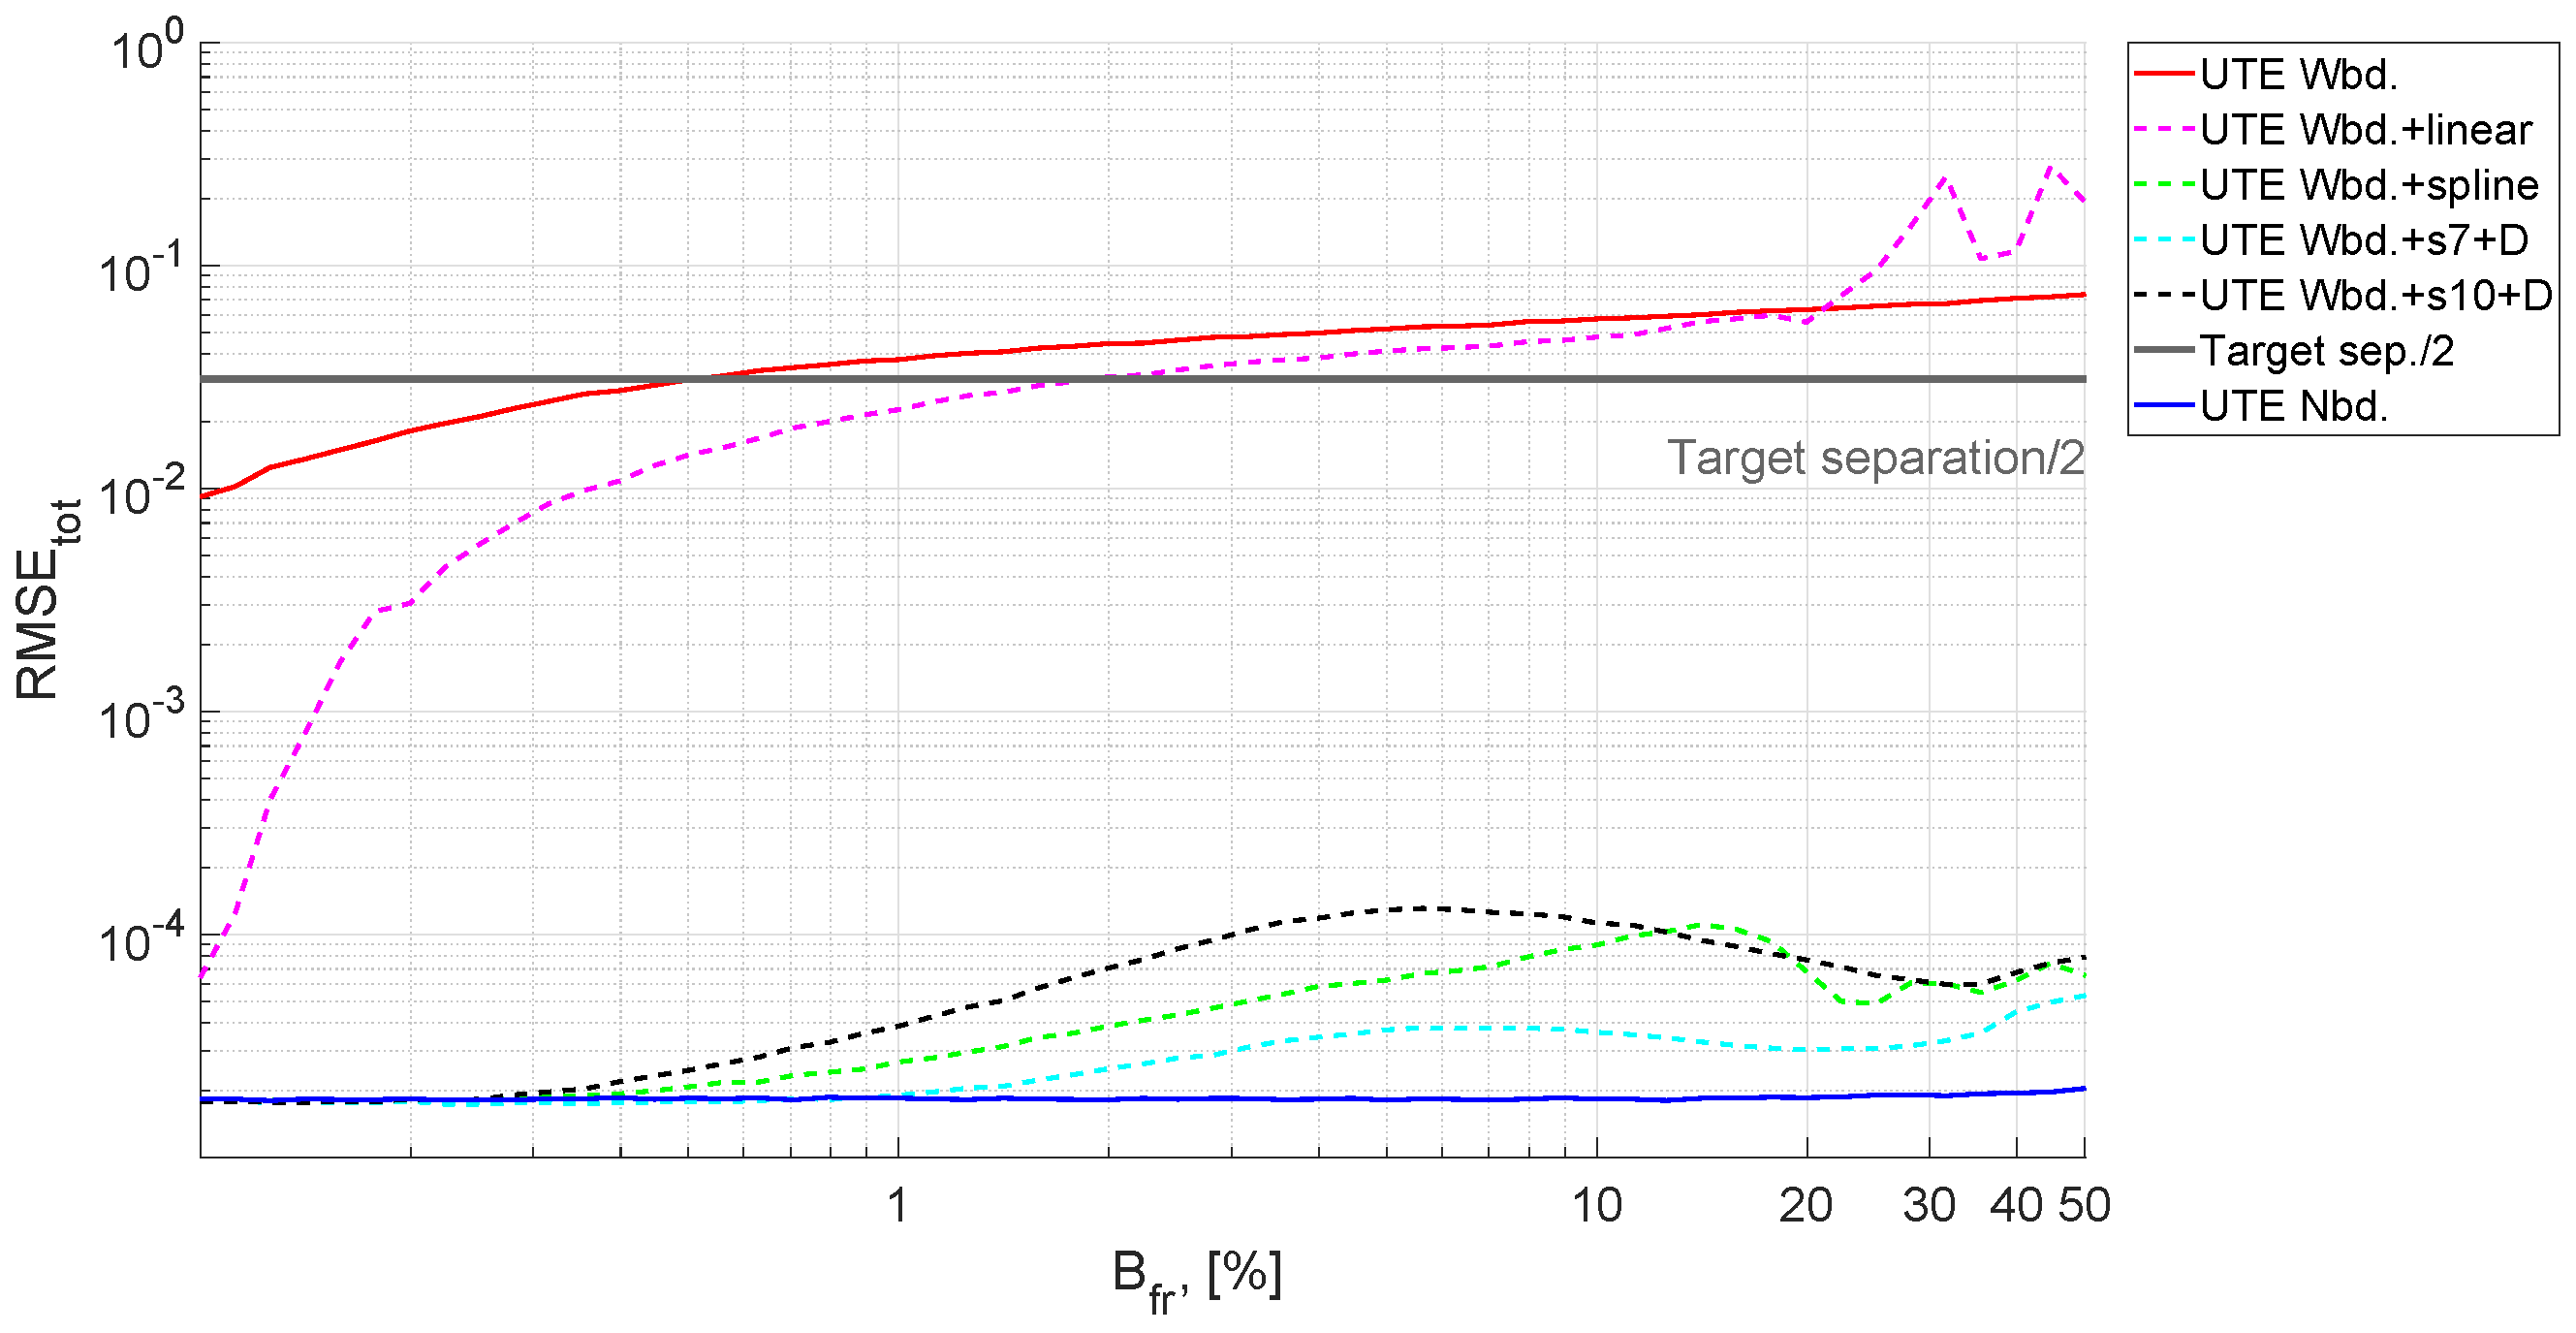
\includegraphics[scale=0.27]{FRAC_ed_final}
	}
	\caption{Среднеквадратическая ошибка оценивания в широкополосной системе.}
	\label{fig:ch2/sec1:frac}
\end{figure}

Например, на рисунке~\ref{fig:ch2/sec1:frac} изображена среднеквадратическая ошибка оценивания параметров канала связи (направлений прихода сигналов, относительной скорости, расстояния) в зависимости от относительной полосы частот системы.

На графике~\ref{fig:ch2/sec1:frac} изображены следующие кривые:
\begin{description}
	\item[<<UTE Nbd.>>] - <<Unitary Tensor Esprit>> алгоритм \cite{Haardt08}, применённый к узкополосной модели (данные сгенерированы при предположении $\sfr\approx\cfr$);
	\item[<<Target.sep./2>>] - половина минимального расстояния между отражателями в пространстве параметров;
	\item[<<UTE Wbd. + ... >>] -  <<Unitary Tensor Esprit>> алгоритм \cite{Haardt08}, применённый к широкополосной модели;
	\item[<<UTE Wbd. + linear >>] - использование линейной интерполяции для предварительной обработки принятых данных;
	\item[<<UTE Wbd. + spline >>] - использование интерполяции кубическими сплайнами для предварительной обработки принятых данных;
	\item[<<UTE Wbd. + s7/10 + D >>] - использование интерполяции сплайнами высокого порядка (7 и 10) для предварительной обработки принятых данных.
\end{description}

Результаты компьютерного моделирования показывают, что использование предварительной обработки с помощью интерполирования позволяет восстановить эффективность узкополосного алгоритма оценивания (UTE, \cite{Haardt08}). Эффективность пред-обработки зависит от величины относительной полосы частот рассматриваемой системы.

\let\pai\gpai

\section{Оценивание параметров каналов связи с отражателями в ближнем геометрическом поле}\label{ch:ch2/sec2}

Алгоритм TeNFiL и анализ его эффективности (диссертация Евгения), граница Крамера-Рао (диссертация Лианы), доработки.

\section{Анализ потенциальных характеристик оценивания параметров каналов связи при наличии негауссовских аддитивных помех}\label{ch:ch2/sec3}

\begin{comment}
Результаты данного раздела доклада были опубликованы в \cite{vakbib1}.

Планомерно растущие вычислительные способности программно-аппаратных комплексов обработки цифровых сигналов позволяют рассматривать всё более сложные модели данных и распределения аддитивных помех. Усложнение моделей задач, помимо повышения требований к вычислительным ресурсам, также несёт в себе потенциал для улучшения качественных показателей систем использующих цифровую обработку сигналов.

Задача оценивания направлений прихода заданного числа сигналов имеет множество приложений в области радиолокации и коммуникаций, а также, ввиду абстрактности и общеприменимости постановки, в сейсмологии, акустике, ультразвуковых измерениях. 

Задача имеет богатую историю в отечественной \cite{TrifShin1986, ManGel2015} и зарубежной \cite{Capon1969} литературе и продолжает оставаться актуальной. Аналитическое решение задачи отсутствует в литературе, поэтому распространение получили эвристические и численные методы решения. Среди первых стоит выделить класс методов подпространства сигналов \cite{Schmidt1986, Roy1989}, использующих спектральные разложения оценок пространственных ковариационных матриц. Для поиска оптимального решения зачастую применяются численные методы, такие как алгоритм IQML \cite{Bresler1985, Bresler1986}, итеративно максимизирующий функцию правдоподобия выборки, а также алгоритмы-производные от алгоритма EM, такие как MODE \cite{Stoica1990}. С точки зрения негауссовских аддитивных помех в литературе рассмотрен случай импульсного аддитивного шума, заданного смесью двух Гауссовских распределений с разными ковариациями \cite{Kozick2000, Kozick2000b}. Другой класс численных методов итеративно ищет оценку подпространства сигналов \cite{Ziskind1988, Bazzi2018}.

Для оценки эффективности этих алгоритмов, ввиду отсутствия других объективных критериев используется граница Крамера-Рао \cite{Cramer1993, KayS.1993}. Для случая аддитивного Гауссового шума выражение границы можно найти в \cite{Stoica1988, Stoica1989a, Stoica1989, Stoica1990a}, для случая импульсного шума выраженного смесью двух Гауссовых компонент с разными мощностями в \cite{Kozick2000, Kozick2000b, Kalyani2012}. Однако аналитический вывод границы Крамера-Рао в общем случае слишком сложен, и для произвольной смеси Гауссовых компонент отсутствует в литературе.

Целью работы в данном разделе являлся сравнительный анализ потенциальных характеристик оценивания параметров канала связи в виде направлений прихода сигналов массивом антенн в условиях различных моделей аддитивной помехи.

Для сравнения потенциальных характеристик используется нижняя граница Крамера-Рао. Для её вычисления предлагается метод вычисления нижней границы Крамера-Рао для произвольных распределений аддитивной помехи, а также проводится моделирование и сравнительный анализ данной границы для различных моделей аддитивной помехи.

Приведённый в данном разделе метод вычисления границы Крамера-Рао в задаче оценивания направлений прихода сигналов для общего выражения распределения аддитивной помехи основывается на алгоритме Монте-Карло, который используется для оценки информационной матрицы Фишера аддитивной помехи. Данная матрица затем используется для вычисления границы Крамера-Рао для оцениваемых параметров. Метод является общеприменимым до тех пор пока имеется возможность генерации отсчётов помехи.


\section{Одиночное изображение}\label{sec:ch2/sec1}

\begin{figure}[ht]
  \centerfloat{
    \includegraphics[scale=0.27]{latex}
  }
  \caption{TeX.}\label{fig:latex}
\end{figure}

Для выравнивания изображения по-центру используется команда \verb+\centerfloat+, которая является во
многом улучшенной версией встроенной команды \verb+\centering+.

\section{Длинное название параграфа, в котором мы узнаём как сделать две картинки с~общим номером и названием}\label{sec:ch2/sect2}

А это две картинки под общим номером и названием:
\begin{figure}[ht]
  \begin{minipage}[b][][b]{0.49\linewidth}\centering
    \includegraphics[width=0.5\linewidth]{knuth1} \\ а)
  \end{minipage}
  \hfill
  \begin{minipage}[b][][b]{0.49\linewidth}\centering
    \includegraphics[width=0.5\linewidth]{knuth2} \\ б)
  \end{minipage}
  \caption{Очень длинная подпись к изображению,
      на котором представлены две фотографии Дональда Кнута}
  \label{fig:knuth}
\end{figure}

Те~же~две картинки под~общим номером и~названием,
но с автоматизированной нумерацией подрисунков:
\begin{figure}[ht]
    \centerfloat{
        \hfill
        \subcaptionbox[List-of-Figures entry]{Первый подрисунок\label{fig:knuth_2-1}}{%
            \includegraphics[width=0.25\linewidth]{knuth1}}
        \hfill
        \subcaptionbox{\label{fig:knuth_2-2}}{%
            \includegraphics[width=0.25\linewidth]{knuth2}}
        \hfill
        \subcaptionbox{Третий подрисунок, подпись к которому
        не~помещается на~одной строке}{%
            \includegraphics[width=0.3\linewidth]{example-image-c}}
        \hfill
    }
    \legend{Подрисуночный текст, описывающий обозначения, например. Согласно
    ГОСТ 2.105, пункт 4.3.1, располагается перед наименованием рисунка.}
    \caption[Этот текст попадает в названия рисунков в списке рисунков]{Очень
    длинная подпись к второму изображению, на~котором представлены две
    фотографии Дональда Кнута}\label{fig:knuth_2}
\end{figure}

На рисунке~\ref{fig:knuth_2-1} показан Дональд Кнут без головного убора.
На рисунке~\ref{fig:knuth_2}\subcaptionref*{fig:knuth_2-2}
показан Дональд Кнут в головном уборе.

Возможно вставлять векторные картинки, рассчитываемые \LaTeX\ <<на~лету>>
с~их~предварительной компиляцией. Надписи в таких рисунках будут выполнены
тем же~шрифтом, который указан для документа в целом.
На~рисунке~\ref{fig:tikz_example} на~странице~\pageref{fig:tikz_example}
представлен пример схемы, рассчитываемой пакетом \verb|tikz| <<на~лету>>.
Для ускорения компиляции, подобные рисунки могут быть <<кешированы>>, что
определяется настройками в~\verb|common/setup.tex|.
Причём имя предкомпилированного
файла и~папка расположения таких файлов могут быть отдельно заданы,
что удобно, если не~для подготовки диссертации,
то~для подготовки научных публикаций.
\begin{figure}[ht]
    \centerfloat{
        \ifdefmacro{\tikzsetnextfilename}{\tikzsetnextfilename{tikz_example_compiled}}{}% присваиваемое предкомпилированному pdf имя файла (не обязательно)
        \input{Dissertation/images/tikz_scheme.tikz}

    }
    \legend{}
    \caption[Пример \texttt{tikz} схемы]{Пример рисунка, рассчитываемого
        \texttt{tikz}, который может быть предкомпилирован}\label{fig:tikz_example}
\end{figure}

Множество программ имеют либо встроенную возможность экспортировать векторную
графику кодом \verb|tikz|, либо соответствующий пакет расширения.
Например, в GeoGebra есть встроенный экспорт,
для Inkscape есть пакет svg2tikz,
для Python есть пакет matplotlib2tikz,
для R есть пакет tikzdevice.

\section{Пример вёрстки списков}\label{sec:ch2/sec3}

\noindent Нумерованный список:
\begin{enumerate}
  \item Первый пункт.
  \item Второй пункт.
  \item Третий пункт.
\end{enumerate}

\noindent Маркированный список:
\begin{itemize}
  \item Первый пункт.
  \item Второй пункт.
  \item Третий пункт.
\end{itemize}

\noindent Вложенные списки:
\begin{itemize}
  \item Имеется маркированный список.
  \begin{enumerate}
    \item В нём лежит нумерованный список,
    \item в котором
    \begin{itemize}
      \item лежит ещё один маркированный список.
    \end{itemize}
  \end{enumerate}
\end{itemize}

\noindent Нумерованные вложенные списки:
\begin{enumerate}
  \item Первый пункт.
  \item Второй пункт.
  \item Вообще, по ГОСТ 2.105 первый уровень нумерации
  (при необходимости ссылки в тексте документа на одно из перечислений)
  идёт буквами русского или латинского алфавитов,
  а второй "--- цифрами со~скобками.
  Здесь отходим от ГОСТ.
    \begin{enumerate}
      \item в нём лежит нумерованный список,
      \item в котором
        \begin{enumerate}
          \item ещё один нумерованный список,
          \item третий уровень нумерации не нормирован ГОСТ 2.105;
          \item обращаем внимание на строчность букв,
          \item в этом списке
          \begin{itemize}
            \item лежит ещё один маркированный список.
          \end{itemize}
        \end{enumerate}

    \end{enumerate}

  \item Четвёртый пункт.
\end{enumerate}

\section{Традиции русского набора}

Много полезных советов приведено в материале
<<\href{http://www.dropbox.com/s/x4hajy4pkw3wdql/wholesome-typesetting.pdf?dl=1\&pv=1}{Краткий курс благородного набора}>> (автор А.\:В.~Костырка).
Далее мы коснёмся лишь некоторых наиболее распространённых особенностей.

\subsection{Пробелы}

В~русском наборе принято:
\begin{itemize}
    \item единицы измерения, знак процента отделять пробелами от~числа:
        10~кВт, 15~\% (согласно ГОСТ 8.417, раздел 8);
    \item \(\tg 20\text{\textdegree}\), но: 20~{\textdegree}C
        (согласно ГОСТ 8.417, раздел 8);
    \item знак номера, параграфа отделять от~числа: №~5, \S~8;
    \item стандартные сокращения: т.\:е., и~т.\:д., и~т.\:п.;
    \item неразрывные пробелы в~предложениях.
\end{itemize}

\subsection{Математические знаки и символы}

Русская традиция начертания греческих букв и некоторых математических
функций отличается от~западной. Это исправляется серией
\verb|\renewcommand|.
\begin{itemize}
%Все \original... команды заранее, ради этого примера, определены в Dissertation\userstyles.tex
    \item[До:] \( \originalepsilon \originalge \originalphi\),
    \(\originalphi \originalleq \originalepsilon\),
    \(\originalkappa \in \originalemptyset\),
    \(\originaltan\),
    \(\originalcot\),
    \(\originalcsc\).
    \item[После:] \( \epsilon \ge \phi\),
    \(\phi \leq \epsilon\),
    \(\kappa \in \emptyset\),
    \(\tan\),
    \(\cot\),
    \(\csc\).
\end{itemize}

Кроме того, принято набирать греческие буквы вертикальными, что
решается подключением пакета \verb|upgreek| (см. закомментированный
блок в~\verb|userpackages.tex|) и~аналогичным переопределением в
преамбуле (см.~закомментированный блок в~\verb|userstyles.tex|). В
этом шаблоне такие переопределения уже включены.

Знаки математических операций принято переносить. Пример переноса
в~формуле~\eqref{eq:equation3}.

\subsection{Кавычки}
В английском языке приняты одинарные и двойные кавычки в~виде ‘...’ и~“...”.
В России приняты французские («...») и~немецкие („...“) кавычки (они называются
«ёлочки» и~«лапки», соответственно). ,,Лапки`` обычно используются внутри
<<ёлочек>>, например, <<... наш гордый ,,Варяг``...>>.

Французкие левые и правые кавычки набираются
как лигатуры \verb|<<| и~\verb|>>|, а~немецкие левые
и правые кавычки набираются как лигатуры \verb|,,| и~\verb|‘‘| (\verb|``|).

Вместо лигатур или команд с~активным символом "\ можно использовать команды
\verb|\glqq| и \verb|\grqq| для набора немецких кавычек и команды \verb|\flqq|
и~\verb|\frqq| для набора французских кавычек. Они определены в пакете
\verb|babel|.

\subsection{Тире}
%  babel+pdflatex по умолчанию, в polyglossia надо включать опцией (и перекомпилировать с удалением временных файлов)
Команда \verb|"---| используется для печати тире в тексте. Оно несколько короче
английского длинного тире. Кроме того, команда задаёт небольшую жёсткую отбивку
от слова, стоящего перед тире. При этом, само тире не~отрывается от~слова.
После тире следует такая же отбивка от текста, как и~перед тире. При наборе
текста между словом и командой, за которым она следует, должен стоять пробел.

В составных словах, таких, как <<Закон Менделеева"--~Клапейрона>>, для печати
тире надо использовать команду \verb|"--~|. Она ставит более короткое,
по~сравнению с~английским, тире и позволяет делать переносы во втором слове.
При~наборе текста команда \verb|"--~| не отделяется пробелом от слова,
за~которым она следует (\verb|Менделеева"--~|). Следующее за командой слово
может быть  отделено от~неё пробелом или перенесено на другую строку.

Если прямая речь начинается с~абзаца, то перед началом её печатается тире
командой \verb|"--*|. Она печатает русское тире и жёсткую отбивку нужной
величины перед текстом.

\subsection{Дефисы и переносы слов}
%  babel+pdflatex по умолчанию, в polyglossia надо включать опцией (и перекомпилировать с удалением временных файлов)
Для печати дефиса в~составных словах введены две команды. Команда~\verb|"~|
печатает дефис и~запрещает делать переносы в~самих словах, а~команда \verb|"=|
печатает дефис, оставляя \TeX ’у право делать переносы в~самих словах.

В отличие от команды \verb|\-|, команда \verb|"-| задаёт место в~слове, где
можно делать перенос, не~запрещая переносы и~в~других местах слова.

Команда \verb|""| задаёт место в~слове, где можно делать перенос, причём дефис
при~переносе в~этом месте не~ставится.

Команда \verb|",| вставляет небольшой пробел после инициалов с~правом переноса
в~фамилии.

\section{Текст из панграмм и формул}

\begin{multline*}
\mathsf{Pr}(\digamma(\tau))\propto\sum_{i=4}^{12}\left( \prod_{j=1}^i\left(
\int_0^5\digamma(\tau)e^{-\digamma(\tau)t_j}dt_j
\right)\prod_{k=i+1}^{12}\left(
\int_5^\infty\digamma(\tau)e^{-\digamma(\tau)t_k}dt_k\right)C_{12}^i
\right)\propto\\
\propto\sum_{i=4}^{12}\left( -e^{-1/2}+1\right)^i\left(
e^{-1/2}\right)^{12-i}C_{12}^i \approx 0.7605,\quad
\forall\tau\neq\overline{\tau}
\end{multline*}

%Большая фигурная скобка только справа
\[\left. %ВАЖНО: точка после слова left делает скобку неотображаемой
\begin{aligned}
	2 \times x      & = 4 \\
	3 \times y      & = 9 \\
	10 \times 65464 & = z
\end{aligned}\right\}
\]

\end{comment}